\section{AFL}

% Talk about why it is state of the art!


American Fuzzy Lop was originally developed by Michal Zalewski. He introduces this open-source project as \say{a security-oriented fuzzer that employs a novel type of compile-time instrumentation and genetic algorithms to automatically discover clean, interesting test inputs that trigger new internal states in the targeted binary. This substantially improves the functional coverage for the fuzzed code. The compact synthesized corpora produced by the tool are also useful for seeding other, more labor- or resource-intensive testing regimes down the road.} \cite{zalewski2014american} AFL can dynamically test a target program and for this purpose, instrumentation is required for better performance of the fuzzer.

\subsection{Stages of fuzzing with AFL}

As our fuzzer is based on AFL, we will walk over the features of AFL that we need for our fuzzer. Based on \ref{fig:fuzz_phases}, AFL has the following phases:

\begin{enumerate}
    \item \textbf{Target identification and setup:}
    The target application for AFL is any executable program. The only limitation of AFL for the target is that the target executable must take a list of at least one input filename as the program's arguments. 
    
    % For instance: -- Example

    % TODO: Introduce the example for target executable in this article

    Hence, it is not a necessity for the program to take only one argument in command line, instead, a driver for AFL can add different techniques of getting input for the program.

    Next action before starting the fuzz testing, is instrumentation. If the insturmentation of the target program is not done yet, AFL doesn't have any technique for fuzzing except dumb fuzzing, which mutates the inputs completely randomly, without considering any information from the program's executions. We will discuss about the instrumentation more in this chapter.
    
    \item \textbf{Identify and setup inputs:}
    The seeds for AFL must be placed in a directory, and AFL puts them in it's queue for fuzzing later. Based on what our fuzzing goals are, preparing a corpora of different seeds with different code coverages, enhances the exploration of AFL to discover more execution paths. AFL can pick a subset of the provided seeds using \codeword{afl-cmin}. This tool \say{tries to find the smallest subset of files in the input directory that still trigger the full range of instrumentation data points seen in the starting corpus}. Instrumentation is mandatory for using \codeword{afl-cmin}. AFL can also minimize test inputs using \codeword{afl-tmin}. \say{The tool works with crashing and non-crashing test inputs alike. In the crash mode, it will happily accept instrumented and non-instrumented binaries. In the non-crashing mode, the minimizer relies on standard AFL instrumentation to make the file simpler without altering the execution path.} \cite{afl_git}

    Another option introduced by AFL is using dictionaries for investigating the possible grammars used in input parsing. As it is described in AFL's documentation, \say{by default, afl-fuzz mutation engine is optimized for compact data formats - say, images, multimedia, compressed data, regular expression syntax, or shell scripts. It is somewhat less suited for languages with particularly verbose and redundant verbiage - notably including HTML, SQL, or JavaScript.
    
    To avoid the hassle of building syntax-aware tools, afl-fuzz provides a way to seed the fuzzing process with an optional dictionary of language keywords, magic headers, or other special tokens associated with the targeted data type - and use that to reconstruct the underlying grammar on the go}

    After providing required or useful corpora of inputs, AFL can start it's fuzz testing. 
    
    % For instance, for our example program, we have:

    % TODO: Use the command for starting AFL on our Example!
    % -- Example afl-fuzz start

    \item \textbf{Generate fuzzed data:}
    As discussed before, AFL is a \textbf{mutation-based} fuzzer, meaning that it generates new inputs by mutating (\textbf{favored}) inputs. 

    \begin{itemize}
        \item \textbf{Favored inputs}: After an input is executed, it's favor factor is calculated and later, if it is still interesting for AFL, it is marked as Favored. AFL finds favorable path (collected using a \textbf{bitmap} after instrumentation) for the purpose of \say{having a minimal set of paths that trigger all the bits seen in the bitmap so far, and focus on fuzzing them at the expense of the rest.} \cite{afl_git} 
        \begin{equation}
            favored\_factor = e.exec\_time \times e.length
        \end{equation}
        
        The preference of AFL for the favored inputs, increases the performance of AFL in finding more crashes, but it is against the effort of finding an input with higher time consumption.

        \item \textbf{Mutation strategies}: In order to generate new inputs, AFL takes a queue of inputs and tries mutating and running each one of them. The mutation strategies are in a queue of different strategies that are run on an input to generate more inputs eventually. These strategies include bit-fliping, byte-fliping, simple arithmatics, known integers, stack tweaks, and test case splicing. \cite{afl_strategies}
        
    \end{itemize}

    \item \textbf{Execute fuzzed data:}
    To simplify, AFL takes an instrumented program, a directory for seeds and a directory for outputs:

    \begin{lstlisting}[language=bash,style=CommandStyle,caption=Execute AFL]
  afl-fuzz -i <in_dir> -o <out_dir> [options] -- /path/to/fuzzed/app [params]
    \end{lstlisting}

    Before running the program using the seeds provided, AFL first looks for favored inputs, in the queue of seeds, then picks the favored one and runs the instrumented program using the input. To monitor the execution of the program, AFL creates a shared memory with the program, and during the execution of the program, this shared memory is filled with information from the instrumentation. The only shared information that AFL keeps is a bitmap of the program's basic blocks, that were visited in the execution. After the execution is finished, AFL processes the bitmap and decides on what the next stage would be. If the program is crashed or hanged, it is kept for exploitability purposes and if the error is unique, it is stored in the output directory. This loop is then repeated for other favored inputs.

    % TODO: mention the algorithm related to AFL

    % \begin{algorithm}[H]
    %     \caption{AFL-FUZZ}
    %     \KwData{instrumented\_program, input\_queue}
    %     initializations();

    %     \While{fuzzing is not terminated}{
    %         favored\_input = find\_favored\_input(input\_queue)\;
    %         new\_seed = mutate(favored\_input)\;
    %         exit\_value = execute(new\_seed, instrumented\_program); \tcp{Update bitmap}
    %         \If{exit\_value!=0}{
    %             ERROR\_ACQUIRED\;
    %         }
    %     }
    % \end{algorithm}

    \item \textbf{Monitor for exceptions:} Beside reporting the crashes and hangs, AFL also logs the information about it's fuzzing stages and stats. In general, AFL provides a \textit{status screen} which has eight different sections:
    
    \begin{figure}[!t]
        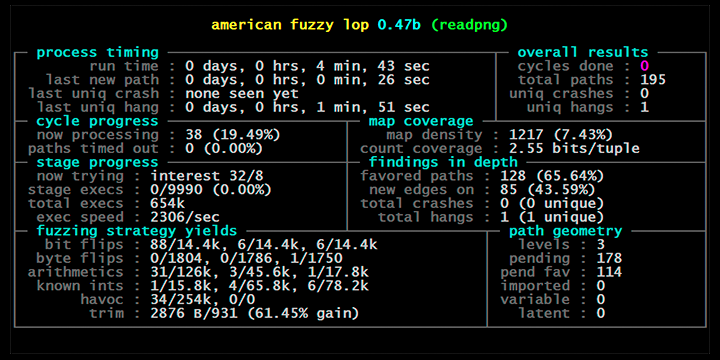
\includegraphics[width=\textwidth]{Chapter2/afl_screen.png}
        \centering
        \caption{AFL status screen}
        \label{fig:status_screen}
    \end{figure} 
    
    
    \begin{enumerate}
        \item \textbf{Process timing}: This section tells about how long the process of fuzzing is running.
        \item \textbf{Overall results}: A simplified information about the progress of AFL in finding paths, hangs and crashes. 
        \item \textbf{Cycle progress}: As mentioned before, AFL takes one input and repeats mutating it for a while. This section shows the information about the current cycle that the fuzzer is working on.
        \item \textbf{Map coverage}: \say{The section provides some trivia about the coverage observed by the instrumentation embedded in the target binary. The first line in the box tells you how many branch we have already hit, in proportion to how much the bitmap can hold. The number on the left describes the current input; the one on the right is the value for the entire input corpus. The other line deals with the variability in tuple hit counts seen in the binary. In essence, if every taken branch is always taken a fixed number of times for all the inputs we have tried, this will read "1.00". As we manage to trigger other hit counts for every branch, the needle will start to move toward "8.00" (every bit in the 8-bit map hit), but will probably never reach that extreme. 
        
        Together, the values can be useful for comparing the coverage of several different fuzzing jobs that rely on the same instrumented binary.
        }
        \item \textbf{Stage progress}: The information about the current mutation stage is briefly provided here.
        \item \textbf{Findings in depth}: The crashes and hangs and any other findings (here we just have the other information about the coverage) are presented in this section.
        \item \textbf{Fuzzing strategy yields}: To illusterate more stats about the strategies used since the beginning of fuzzing, and for comparison of those strategies, AFL keeps track of how many paths were explored, in proportion to the number of executions attempted, for each of the fuzzing strategies.
        \item \textbf{Path geometry}: The information about the inputs and their depths, which says how many generations of different paths were produced in the process. For instance, we call the seeds we provided for fuzzing, the "level 1" inputs. Next, a new set of inputs is generated as the "level 2", the inputs derived from "level 2" are "level 3" and so on.
    \end{enumerate}

    \item \textbf{Exploitability:} Figuring out whether the crashes and hangs are exploitable or not, is an important stage for exposing and exploiting the vulnerabilities. AFL provides another automated tool for checking the inputs responsible for the faults and mutating those inputs in order to find a more problematic input. To use this tool, we have to provide \textbf{-C} option for afl-fuzz:
    
    \begin{lstlisting}[language=bash,style=CommandStyle,caption=AFL Crash Triage]
afl-fuzz -C -i <in_dir> -o <out_dir> [options] -- /path/to/fuzzed/app [params]
    \end{lstlisting}

    If we define the input directory as the directory of the crashes, then AFL starts it's crash exploration, by looking for other inputs with different paths, but the same state. 

    Another technique for assessing the exploitability manually, is to use a debugger and investigate the causes of the crashes/hangs.
    
\end{enumerate}


% What is AFL and what are the AFL approaches for stages of fuzzing
% Important feature of AFL for us
% Talk about instrumentation and LLVM


